% \documentclass[final,5p,times,twocolumn]{elsarticle}
% %\documentclass[preprint,review,12pt]{elsarticle}
% \usepackage{hyperref} %% optional
% \usepackage{amssymb}
% \usepackage{amsmath}
% \biboptions{compress}
% 
% \newcounter{bla}
% \newenvironment{refnummer}{%
% \list{[\arabic{bla}]}%
% {\usecounter{bla}%
%  \setlength{\itemindent}{0pt}%
%  \setlength{\topsep}{0pt}%
%  \setlength{\itemsep}{0pt}%
%  \setlength{\labelsep}{2pt}%
%  \setlength{\listparindent}{0pt}%
%  \settowidth{\labelwidth}{[9]}%
%  \setlength{\leftmargin}{\labelwidth}%
%  \addtolength{\leftmargin}{\labelsep}%
%  \setlength{\rightmargin}{0pt}}}
%  {\endlist}
% 
% 
% \journal{Computer Physics Communications}
% 
% \begin{document}
% 
% \begin{frontmatter}
% 
\chapter{Mapping algorithm from the two-dimensional aperiodic Thue-Morse structure to the square lattice}
\label{chap:TM_to_TB}
\label{paper:5_start}

\begin{center}
Ben Payne$^1$, Heeso Noh$^2$, Hui Cao$^2$, and Alexey Yamilov$^1$                                                                               \end{center}

\ \\
% \author[a]{Ben Payne\corref{author}}
% \author[b]{Heeso Noh}
% \author[b]{Hui Cao}
% \author[a]{Alexey Yamilov}
\begin{center}
\textit{$^1$Department of Physics, Missouri University of Science \& Technology,\\ Rolla, MO 65409\\
$^2$Department of Applied Physics, Yale University, New Haven, CT 06520}\end{center}

\ \\
% 
% \cortext[author] {Corresponding author.\\\textit{E-mail address:} benjamin.payne@mst.edu}
% \address[a]{Department of Physics, Missouri University of Science \& Technology, Rolla, Missouri 65409, USA}
% \address[b]{Department of Applied Physics, Yale University, New Haven, Connecticut 06520-8482, USA}
% 
% \begin{abstract}
\addcontentsline{toc}{section}{ABSTRACT}
\begin{center}\textbf{ABSTRACT\footnote{In preparation for Journal of Physics A (2012).}}        \end{center}

Deterministic aperiodic structures, such as those obtained via the Thue-Morse algorithm, exhibit a variety of unusual transport properties not found in either ordered or random media. The non-periodic nature of this system makes it notoriously difficult to characterize theoretically, especially in dimensions higher than one. Here, we demonstrate the possibility of mapping the two-dimensional aperiodic Thue-Morse pattern of micro-cavities onto a square lattice, making it easily amenable to the tight-binding description. We also show that only three distinct nearest and three next-nearest micro-cavity arrangements exist. An implementation of this mapping procedure in Matlab is provided. 
% \end{abstract}
% 
% \begin{keyword}
% Aperiodic structure \sep Thue-Morse sequence
% \end{keyword}
% 
% \end{frontmatter}

% {\bf PROGRAM SUMMARY}
% 
% \begin{small}
% \noindent
% {\em Manuscript Title:} Mapping algorithm from the two-dimensional aperiodic Thue-Morse structure to the square lattice \\
% {\em Authors:} Ben Payne, Heeso Noh, Hui Cao, Alexey Yamilov                      \\
% {\em Program Title:} thuemorse\_to\_square\_mapping\\
% {\em Journal Reference:}                                      \\
% {\em Catalogue identifier:}                                   \\
% {\em Licensing provisions:} Common                         \\
% {\em Programming language:}  Matlab \\ % tested with Matlab 7.10.0.499 (R2010a)
% {\em Computer:} personal computer running Matlab      \\
% {\em Operating system:} Operating system sufficient to run Matlab   \\
% {\em RAM:} 1 Gigabyte                                              \\
% {\em Keywords:} Aperiodic structure, Thue-Morse sequence  \\
% {\em Classification:} 7.9 Transport Properties, 18 Optics            \\
% {\em Nature of problem:} The Thue-Morse algorithm generates a two-dimensional (2D) binary array which is not translationally invariant. This pattern can be used to fabricate an aperiodic 2D array of optical micro-cavities. We show this array can be reduced to a square (periodic) lattice, making possible the application of powerful theoretical analysis based on the tight-binding description.  \\
% {\em Solution method:} By identifying underlying structure in the 2D Thue-Morse sequence, we demonstrate the possibility of mapping onto the 2D square lattice with a finite set of local coupling arrangements. \\
% {\em Restrictions:} The maximum size of the resulting array is limited by computer memory. Input parameter generation $g$ with values from 5 to 12 have been tested, which result in arrays of size $2^5$ to $2^{12}$, respectively. \\
% {\em Unusual features:} None.\\
% {\em Additional comments:} None.\\
% {\em Running time:} Less than 3 minutes on current desktop computers (Intel Pentium 4 3.2Ghz CPU, 4GB RAM). \\
% \end{small}


\section{INTRODUCTION}
\label{sec:introduction_mapping}

Deterministic aperiodic structures (DAS)~\cite{2009_Barber} lie between periodic and random, ranging from quasi-crystals to pseudo-random arrangements. Unlike crystals, they do not have translational symmetry. In contrast with random media, DAS are defined by mathematical rules and have long-range order. {\it Photonic} deterministic aperiodic nano-structures can now be routinely prepared with a variety of nano-fabrication techniques~\cite{2011_Dal_Negro_DAS_review}.

An exhaustive classification of quasi-periodic and aperiodic systems can be accomplished based on an analysis of the structure factor~\cite{2010_Ivchenko}. Quasiperiodic (e.g.~Fibonacci sequence) arrangements are characterized by a pure point spectrum. Exhibiting higher levels of complexity, aperiodic structures can be further subdivided into those having either a singular continuous spectrum or an absolutely continuous spectrum~\cite{2006_Macia}. The prominent example in the former class is the Thue-Morse~\cite{1921_Morse} sequence -- the focus of this study. 
 
Previous studies of Thue-Morse structures revealed highly anomalous transport properties and unusual energy spectra with self-similar features~\cite{1988_Cheng_Thue_Morse,1989_Luck}. One-dimensional (1D) photonic Thue-Morse structures~\cite{1997_Liu,2004_Negro,2004_Qiu,2005_Agarwal,2005_Joannopoulos,2007_Agarwal} are amenable to a variety of theoretical treatments~\cite{2009_Barber,2010_Ivchenko}. Higher dimensional structures are predicted to display richer behaviors~\cite{2011_Dal_Negro_DAS_review}, just as wave transport in two-dimensional~(2D) random media is more complicated than in~1D~\cite{1979_Anderson}. This observation is indeed supported by the theoretical~\cite{2007_Moretti,2008_Boriskina} and  experimental studies on 2D Thue-Morse DAS that recently appeared in literature~\cite{2004_Negro,2007_Agarwal,2009_Boriskina,2007_Matsui,2008_Gopinath_DAS,2011_Cao_DAS}. Despite the practical interest in the 2D systems, the increased complexity (compared to the 1D counterparts) limits the availability of analytical approaches. The tight binding approximation is generally unavailable in photonic systems, contributing to the problem.

Two-dimensional Thue-Morse DAS can be created by selectively removing particles from a 2D square lattice~\cite{2011_Dal_Negro_DAS_review,2008_Gopinath_DAS}. This process generates a pattern of~$2\times2$ micro-cavities, c.f.~Fig.~\ref{fig:mapping_procedure}, which exhibits self-similar structure on progressively larger scales. These micro-cavities can support confined modes~\cite{2007_Moretti,2008_Boriskina}, similar to whispering gallery modes of micro-disk resonators. Patterns of coupling between the cavity modes in the Thue-Morse structure plays an important role in determining the lasing mode profile~\cite{2011_Cao_DAS}. 

The goal of this work is to demonstrate the possibility of mapping the micro-cavity array in the 2D aperiodic Thue-Morse structure onto a square lattice. We provide a Matlab numerical code which identifies {\it exactly four nearest and four next-nearest neighbors of each cavity}. It is demonstrated that only three types of neighboring arrangements exist in the Thue-Morse structure, allowing assignment of nearest and next-nearest neighbor coupling coefficients to each micro-cavity. Thus, we accomplish the reduction of 2D {\it aperiodic} Thue-Morse array to the {\it periodic} square array of micro-cavities with {\it aperiodic couplings}. Our finding opens up the possibility of a thorough theoretical investigation based on the tight binding Hamiltonian description~\cite{2009_Barber}.

\begin{figure}%[h]
\begin{flushleft} 
%\begin{Large}
\ \ \ (a)
%\end{Large}
\end{flushleft}
\vskip -0.3in
\centering{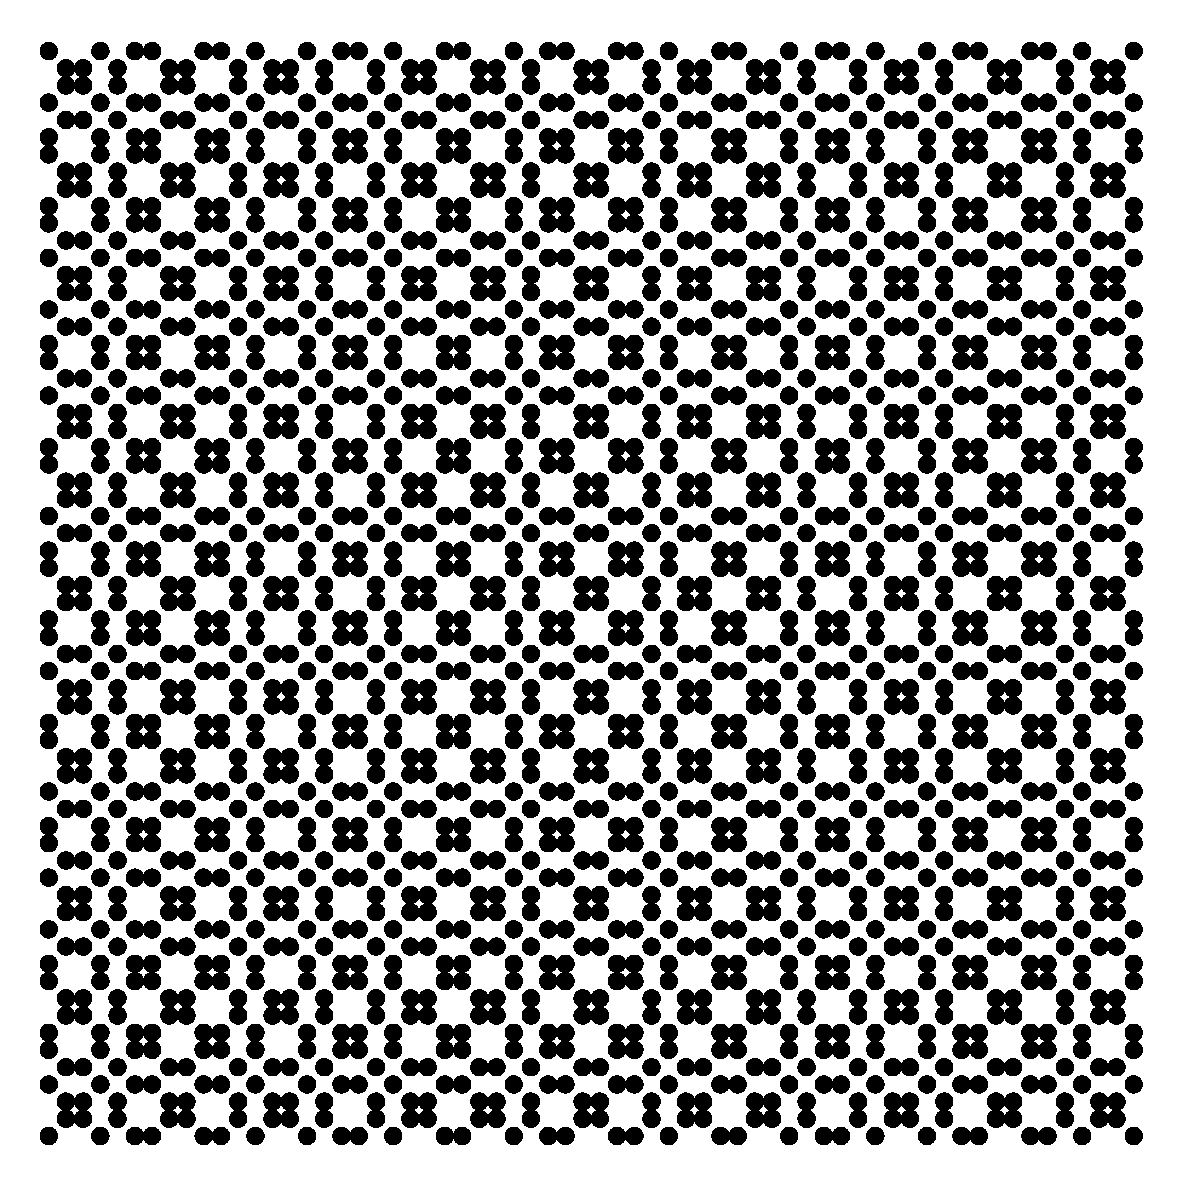
\includegraphics[width=2.4in,angle=0]{chapters/Mapping_algorithm_from_the_two-dimensional_aperiodic_Thue-Morse_structure_to_the_square_lattice/pictures/fig1a_TM_2D_gen6_scatterers_dots}}
\begin{flushleft} 
%\begin{Large}
\ \ \ (b)
%\end{Large}
\end{flushleft}
\vskip -0.2in
\centering{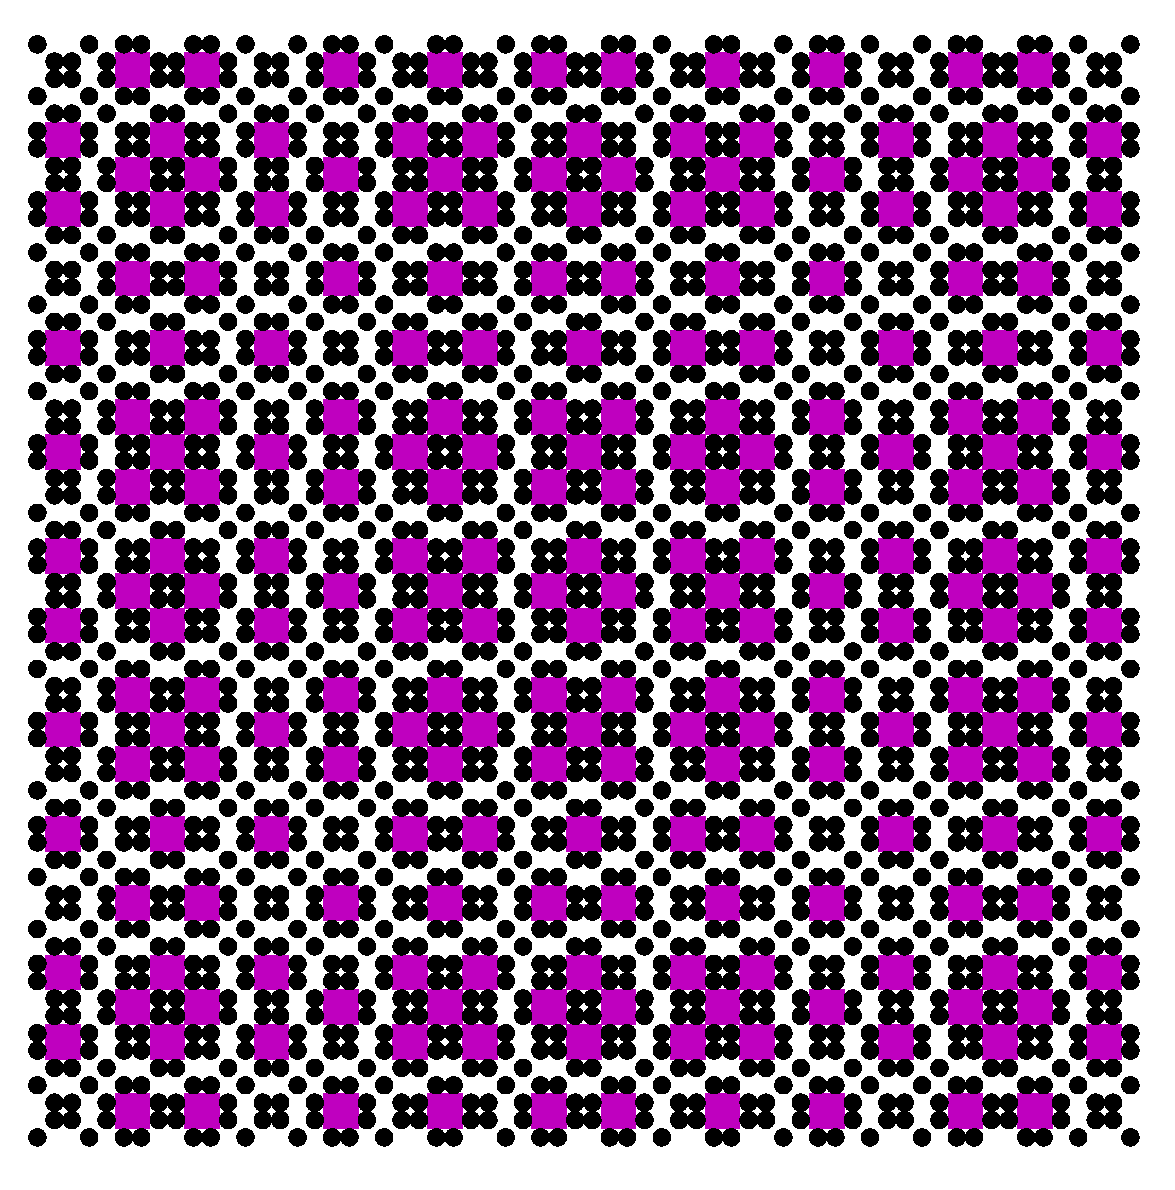
\includegraphics[height=2.4in,angle=0]{chapters/Mapping_algorithm_from_the_two-dimensional_aperiodic_Thue-Morse_structure_to_the_square_lattice/pictures/fig1b_TM_2D_gen6_scatterers_with_squares}}
\begin{flushleft} 
%\begin{Large}
\ \ \ (c)
%\end{Large}
\end{flushleft}
\vskip -0.2in
\centering{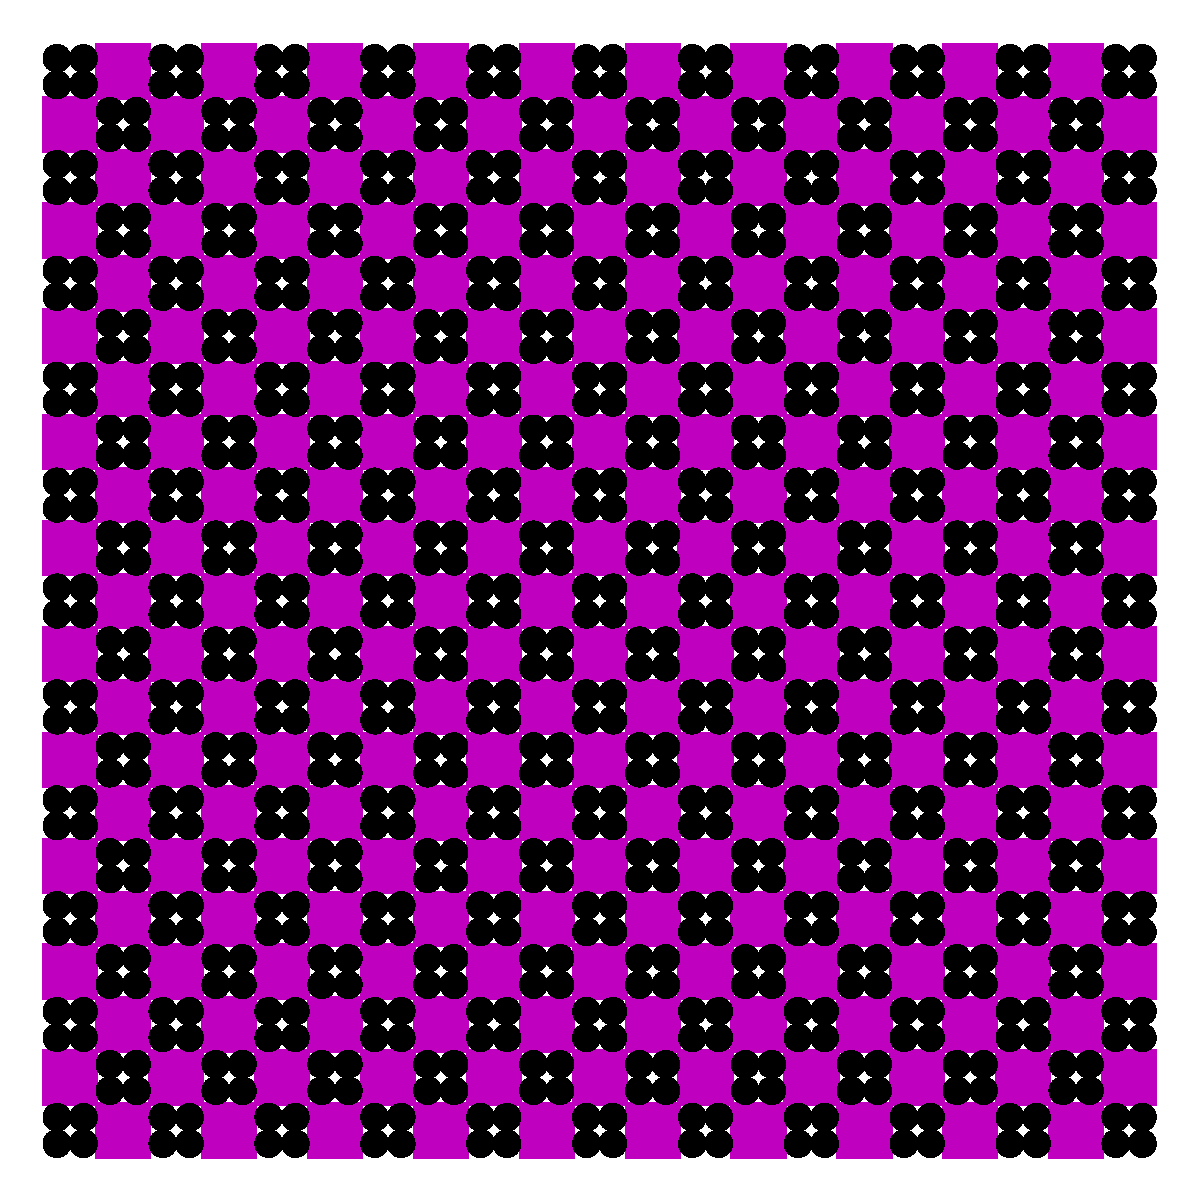
\includegraphics[width=1.5in,angle=0]{chapters/Mapping_algorithm_from_the_two-dimensional_aperiodic_Thue-Morse_structure_to_the_square_lattice/pictures/fig1c_TM_2D_gen6_scatterers_collapsed}}
\caption[(a)~The 2D Thue-Morse structure of generation $g=6$~($64\times64$ elements).]{\label{fig:mapping_procedure} (a)~The 2D Thue-Morse structure of generation $g=6$~($64\times64$ elements). After populating the 2D square lattice with binary elements~$A$ and~$B$ via the inflation procedure $A\rightarrow AB$ and $B\rightarrow BA$; $A$~is interpreted as the positions of scatters. (b)~Same as~(a) with the $2\times2$ clusters regions void of scatters highlighted. These regions play the role of optical micro-cavities in the experiment~\cite{2011_Cao_DAS}. (c) The array of micro-cavities in (b) after the collapse procedure of removing rows and columns void of cavities, see text. The collapsed structure is a periodic square lattice rotated by $45^\circ$; it facilitates identification of the neighboring cavities.}
\end{figure}

\section{MAPPING MICRO-CAVITIES IN 2D THUE-MORSE ARRAY \\ONTO SQUARE LATTICE}

Construction of the 2D Thue-Morse pattern is accomplished in two steps \cite{2008_Negro}. {\it Step~1:} The 1D Thue-Morse sequence is generated by starting with letter~$A$ (generation $g=0$) and repeatedly applying the inflations rules $A\rightarrow AB$ and $B\rightarrow BA$. After repeating the procedure $g$ times the number of elements in the binary sequence is~$2^g$. The complimentary system is defined as $A\rightarrow B$ and $B\rightarrow A$. {\it Step~2:} Using the~$2^g$ elements of the 1D sequence obtained in Step~1 as seeds, we build 1D Thue-Morse sequences of $g$'th generation along the second dimension of the structure. $A$~elements in the resulting~$2^g\times2^g$ array define the position of the ``particles,'' e.g.~cylindrical holes in a dielectric membrane~\cite{2011_Cao_DAS}.  
%\href{http://mathworld.wolfram.com/Thue-MorseSequence.html}{Mathworld figure}

Figure~\ref{fig:mapping_procedure}(a) shows the 2D Thue-Morse structure with $g=6$ obtained using the above procedure. We observe the occurrence of micro-cavities formed at the places missing $2\times2$ holes. Holes surrounding a cavity in the dielectric membrane~\cite{2011_Cao_DAS} create a mismatch in the effective refractive index between the inside and outside regions. Hence, the micro-cavity regions can support cavity modes and play an important role in determining transport properties of the system~\cite{2007_Moretti,2008_Boriskina}. 

Figure~\ref{fig:mapping_procedure}(b) highlights the cavity regions in the 2D Thue-Morse structure. The cavities occur only in the columns with identical adjacent seeds, c.f. Step~1 in the construction procedure above. Indeed, by construction, the columns generated from a pair of dissimilar seeds (i.e. $\ldots AB \ldots$ or $\ldots BA \ldots$) can never contain $2\times2$ clusters. The same argument can also be made regarding the rows in the pattern depicted in Fig.~\ref{fig:mapping_procedure}. Hence, the following {\it collapse procedure} can be performed: one drops all columns and all rows void of the $2\times2$ clusters. The result of this operation is a perfectly periodic square lattice of cavities rotated by $45^\circ$, c.f. Fig.~\ref{fig:mapping_procedure}(c). In this state one can {\it uniquely} identify exactly four nearest and four next-nearest neighbors of each cavity. In the next section, we revert to the original structure {\it expansion procedure} to study the patterns in arrangements of the neighbors.

\section{EXHAUSTIVE ENUMERATION OF INTER-CAVITY ARRANGEMENTS}

\begin{figure}%[h]
% \begin{flushleft}
% \begin{Large}
% (a)\hskip 1.5in (b)
% \end{Large}
% \end{flushleft}
%\vskip -0.3in
\centering{
(a) \hskip 0.2in
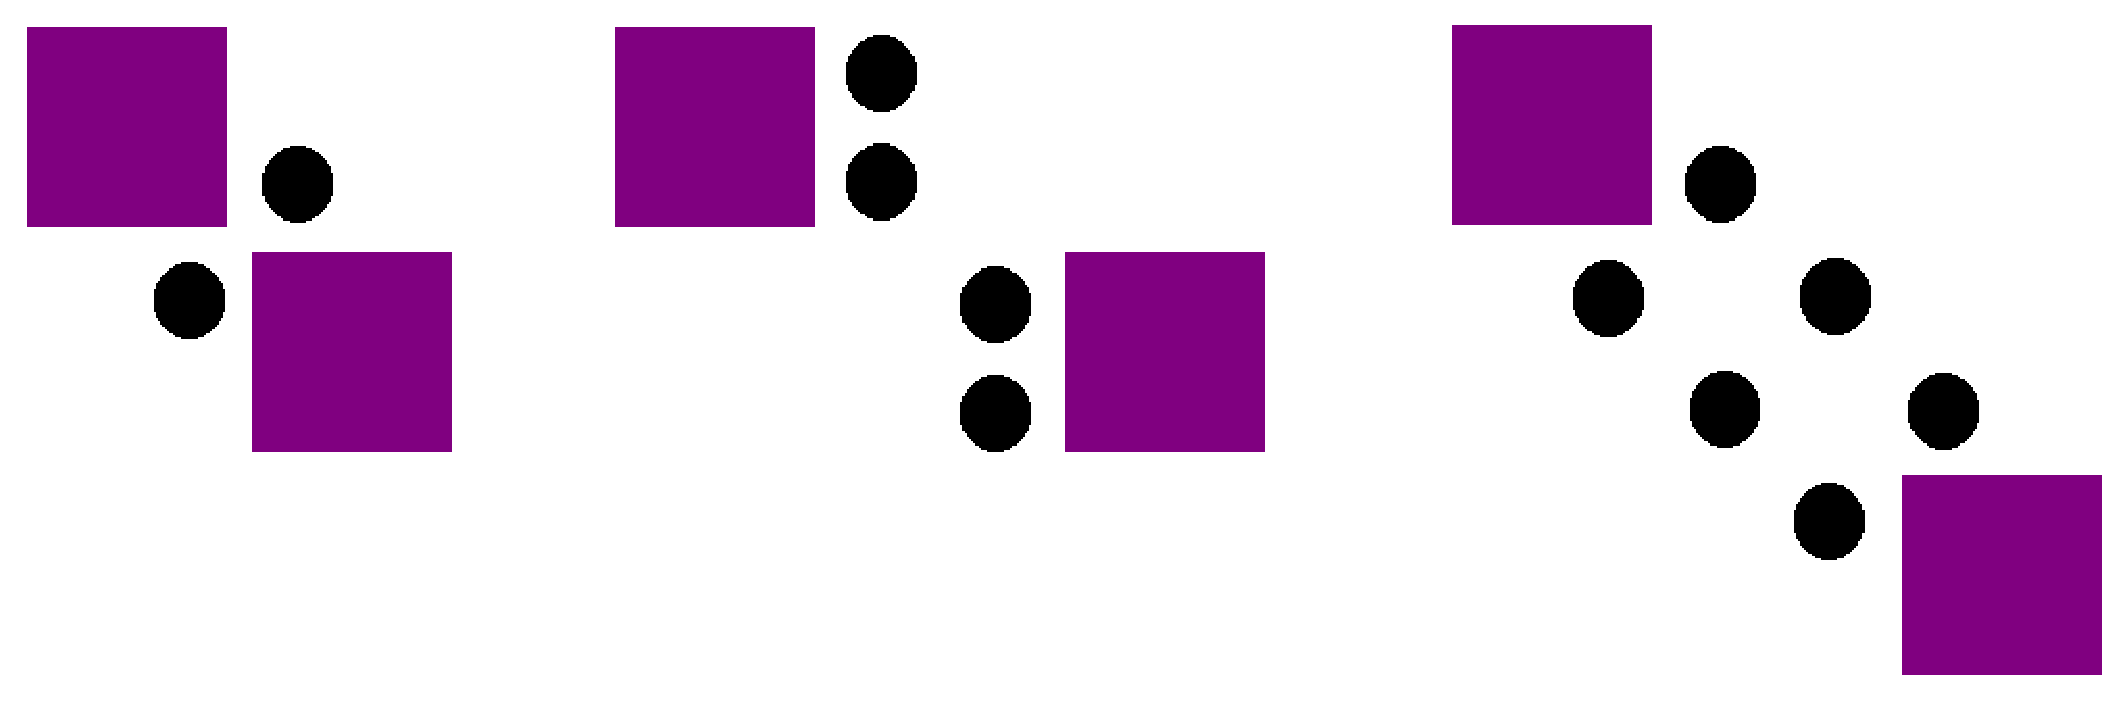
\includegraphics[scale=0.13,angle=0]{chapters/Mapping_algorithm_from_the_two-dimensional_aperiodic_Thue-Morse_structure_to_the_square_lattice/pictures/fig2a_TM_2D_scatterers_purple_nearest_neighbor_couplings}
%\hskip 0.3in
 \hskip 0.2in (b)  \hskip 0.2in
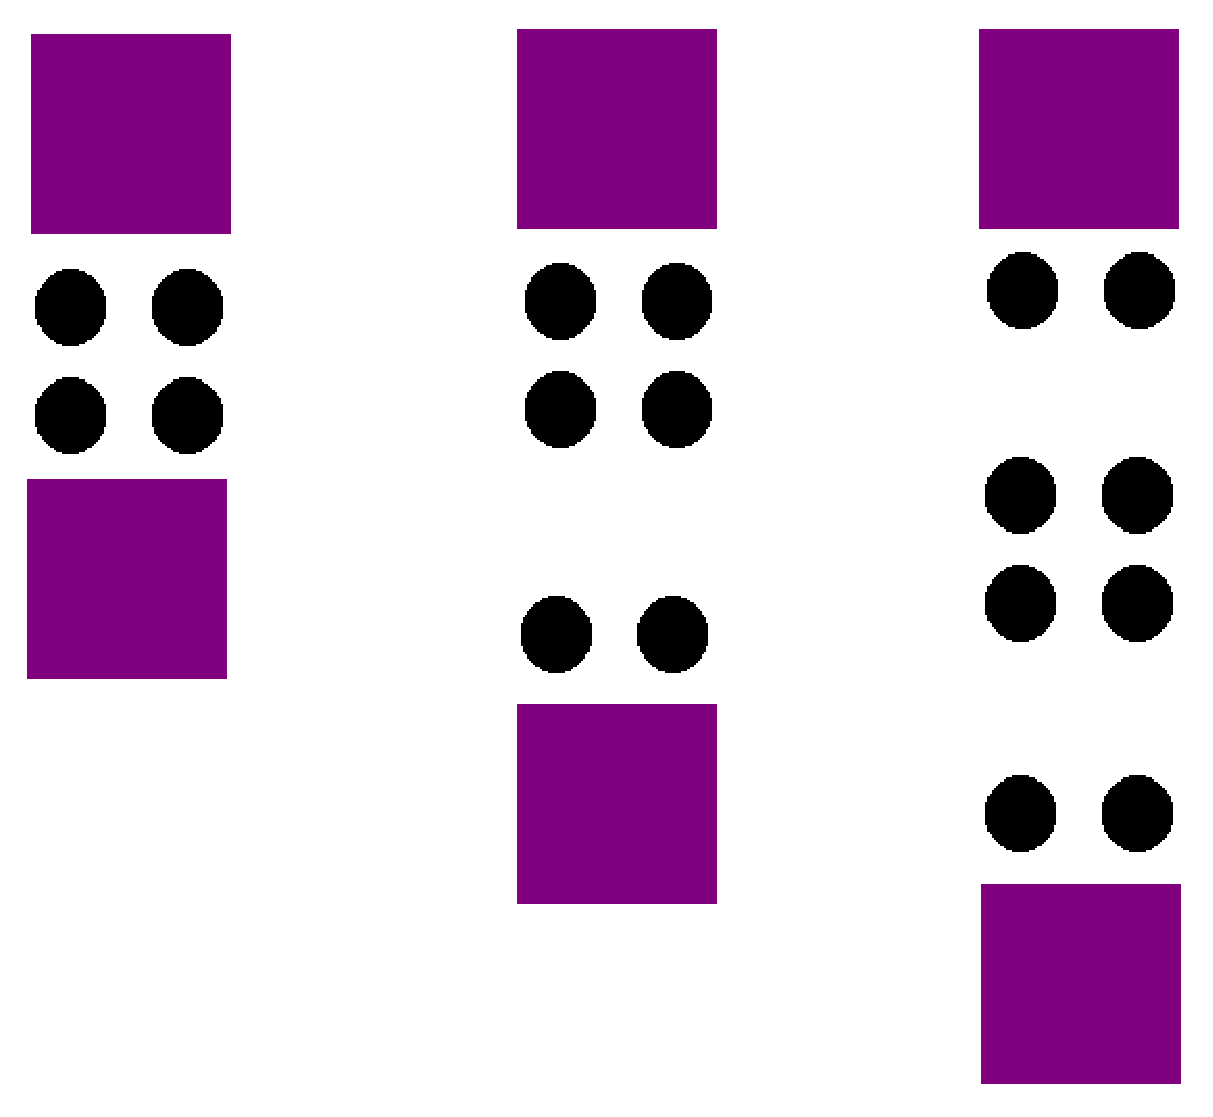
\includegraphics[scale=0.13,angle=0]{chapters/Mapping_algorithm_from_the_two-dimensional_aperiodic_Thue-Morse_structure_to_the_square_lattice/pictures/fig2b_TM_2D_scatterers_purple_next-nearest_neighbor_couplings}}
\caption[(a) Nearest neighbor and (b) next-nearest neighbor arrangements of micro-cavities in 2D Thue-Morse pattern.]{\label{fig:nn_and_nnn_couplings} (a) Nearest neighbor and (b) next-nearest neighbor arrangements of micro-cavities in 2D Thue-Morse pattern. The identification of a neighboring cavity is based on Fig.~\ref{fig:mapping_procedure}c and the coupling type is determined from Fig.~\ref{fig:mapping_procedure}b.}
\end{figure}

After identifying neighboring cavities in the previous section,~c.f. Fig.~1(c), we now turn to the analysis of coupling. The collapse procedure introduced above demonstrates that the furthest separation between next nearest neighbors is equal to six (in the units of lattice constant of the original structure). This observation, and the fact that the Thue-Morse structure by construction contains a finite number of distinct blocks of a given size, leads to the conclusion that the number of distinct cavity couplings should also be finite. Indeed, we find that there are only three distinct nearest and three distinct next-nearest neighbor configurations, c.f.~Fig.~\ref{fig:nn_and_nnn_couplings}~and~\ref{fig:couplings_Hamiltonian}. All cavity configurations can be obtained from these sets by rotation or mirror symmetry transformations. 

The physical significance of a finite number of cavity neighbor arrangements in the Thue-Morse structure is that it results in a finite number of inter-cavity couplings in the tight binding description of the system. The tight-binding model~\cite{1954_Slater_tightBinding} has been a powerful tool in studies of DAS~\cite{2009_Barber}. The Thue-Morse pattern has been treated with the tight-binding model in 1D, where neighbors are clearly defined~\cite{1995_Carpena}. Applying the tight-binding model in 2D is expected to be a fruitful approach in describing transport in the Thue-Morse system~\cite{2011_Cao_DAS}. At the eigenfrequency of the cavity mode, transport is dominated by the coupling between microcavities. Thus, we write
\begin{equation}
E_0\ \psi_{ij}+\sum_{i^\prime j^\prime}c_{ij,i^\prime j^\prime}\ \psi_{i^\prime j^\prime}=E\ \psi_{ij},
\label{eq:2D_array_sites}
\end{equation}
where $E_0$ is the energy of an isolated cavity and $\psi_{ij}$ is the field amplitude of the $ij$'th cavity. Indices $i$ and $j$ enumerate the cavities based on the collapse procedure shown in Fig.~\ref{fig:mapping_procedure}(c). Further, $c_{ij,i^\prime j^\prime}$ denote the couplings between the cavities located at $ij$ and $i^\prime j^\prime$. The analysis of physical proximity in the Thue-Morse structure, c.f.~Fig.~\ref{fig:mapping_procedure}(b), allows us to limit the consideration to two types of coupling -- nearest ($i^\prime=i\pm1$ and $j^\prime=j$, or $i^\prime=i$ and $j^\prime=j\pm1$) and next-nearest ($i^\prime=i\pm1$ and $j^\prime=j\pm1$) couplings only. From Fig.~\ref{fig:nn_and_nnn_couplings} it follows that $c_{ij,i^\prime j^\prime}$ can take one of only six possible values, three of each type. This constitutes the main result of this work. As an example, we used the numerical code described in the next section to generate the color-coded pattern of nearest and next-nearest couplings (four of each type) for the 2D Thue-Morse structure of generation~$g=6$, c.f.~Fig.~\ref{fig:couplings_Hamiltonian}. Thus, the structural complexity in the arrangement of cavities in the original pattern has been reduced to the complexity in connectivities between the elements of the ordered array in Eq.~(\ref{eq:2D_array_sites}).

\begin{figure}%[h]
\begin{flushleft}
%\begin{Large}
(a)
%\end{Large}
\end{flushleft}
\vskip -0.1in
\centering{\includegraphics[width=3.5in]{chapters/Mapping_algorithm_from_the_two-dimensional_aperiodic_Thue-Morse_structure_to_the_square_lattice/pictures/fig3a_nn_color_coded_no_labels_bw_no_colorbar}}
\begin{flushleft}
%\begin{Large}
(b)
%\end{Large}
\end{flushleft}
\vskip -0.1in
\centering{\includegraphics[width=3.5in]{chapters/Mapping_algorithm_from_the_two-dimensional_aperiodic_Thue-Morse_structure_to_the_square_lattice/pictures/fig3b_nnn_color_coded_no_labels_bw_no_colorbar}}
\caption[Four corners of each cavity represent four nearest (a) or four next-nearest (b) couplings of the $2\times 2$ micro-cavities in the 2D Thue-Morse array of generation $g=6$.]{\label{fig:couplings_Hamiltonian} Four corners of each cavity represent four nearest (a) or four next-nearest (b) couplings of the $2\times 2$ micro-cavities in the 2D Thue-Morse array of generation~$g=6$. The results are obtained using the provided Matlab code.}
\end{figure}

\section{DESCRIPTION OF MATLAB CODE}

The supplied code is an implementation of the described algorithm in the Matlab scripting language. Inputs to the primary function are the generation~$g$, complementarity, and a boolean for creating plots. The generation of the Thue-Morse pattern must be a positive integer; values of~$g$ up to 12 have been verified. However, when~$g$ is less than~5 the pattern is too small to show nearest neighbor coupling. The second input, complementarity, allows one to generate the standard Thue-Morse pattern or its complimentary obtained by simultaneous replacement $A\rightarrow B$ and $B\rightarrow A$ throughout the pattern~-- values 0~or~1 respectively. The last input parameter is a boolean switch defining whether or not to generate graphical representations of the results and takes values 0~or~1. After input values are specified by the user, the 2D Thue-Morse pattern is created. The initial size is a square with sides of length~$2^g$. 

For each site in the 2D array, the surrounding pattern is used to determine whether the site is part of a micro-cavity, or if it is part of the buffer in one of three nearest neighbor coupling arrangements. The specific local pattern of the neighboring sites for any given site has only four possible outcomes, the result of which is stored to a three dimensional array of size $2^g\times2^g\times6$. The first layer has four possible values to denote whether a site is part of a micro-cavity or one of the three nearest-neighbor coupling types. The second of the six layers describes whether a site within a $2\times 2$ microcavity is locally in the top, left, right, or bottom position. In the third layer, the nearest neighbor coupling type is recorded for each micro-cavity, c.f.~Fig.~\ref{fig:nn_and_nnn_couplings}a, and the next-nearest coupling type is in the fourth layer of the storage array. Lastly, the original~$x$ and~$y$ coordinates of each site are in the fifth and sixth layers, respectively. 

To determine next-nearest neighbor coupling, micro-cavities sufficiently far from the edges of the 2D array are found. Then, for each micro-cavity, the four next-nearest neighbors are located based on the site arrangement, c.f.~Fig.~\ref{fig:nn_and_nnn_couplings}b, similar to the nearest neighbor procedure above. This result is recorded in layer four of the storage array.

At this stage, all relevant information has been determined. Next, only rows and columns containing micro-cavities are retained, whereas the edges of the 2D Thue-Morse system containing neither nearest nor next-nearest neighbors are discarded. Two arrays, each of size $2^g\times 2^g$, are returned by the main function. These arrays specify nearest and next-nearest coupling types, respectively. 

\section{CONCLUSION}

In this work, we demonstrated the possibility of mapping the array of micro-cavities in the 2D Thue Morse deterministic aperiodic system onto a periodic square lattice. Such mapping allowed us to uniquely identify and exhaustively enumerate the configurations of nearest and next-nearest neighbors. We found that only three configurations of each type exist. Thus, we accomplished the reduction of the original aperiodic structure to the periodic structure with aperiodic arrangement of the limited set of pairings. We developed and provided with this paper a Matlab simulation code which performs this cavity identification and mapping procedure. The results will be used for future investigations of novel transport properties expected in 2D DAS structures. 

\section{ACKNOWLEDGEMENTS}

Authors acknowledge support by National Science Foundation under Grants No. DMR-0704981 and No. DMR-0808937.
% 
% \bibliographystyle{elsarticle-num}
% \bibliography{../../Bibliography/latex_bibliography}
% 
% \end{document}


 